\chapter{CodFS Design}
\label{chap:codfs}

In this chapter, we propose a new parity update approach which reduces the disk
seek overhead of \PL presented in \S~\ref{sec:parity_background}. We then move
to discuss the design and implementation of CodFS, which is an erasure-coded
clustered storage that supports efficient update and recovery.

\section{Parity Update Approach}
\label{sec:parity}

Data updates in erasure-coded clustered storage systems introduce performance
overhead, since they also need to update parity chunks for consistency.  We
consider a deployment environment where network transfer and disk I/O are
performance bottlenecks.  Our goal is to design a parity update scheme that
effectively mitigates both network transfer overhead and number of disk seeks.

In this section, we propose a new delta-based approach called {\bf parity-logging with reserved
space (\PLR)}, which further mitigates fragmentation and reduces the disk seek
overhead of \PL in storing parity deltas.  The main idea is that the storage
nodes reserve additional storage space next to each parity chunk for keeping 
parity deltas.  This ensures that each parity chunk and its parity deltas
can be sequentially retrieved. While the idea is simple, the challenging
issues are to determine (1) the appropriate amount of reserved space to be
allocated when a parity chunk is first stored and (2) the appropriate time
when unused reserved space can be reclaimed to reduce the storage overhead. 

%Subsequent deltas are logged in the reserved space. Once the reserved space
%for a parity chunk is full, the storage node takes a merge operation,
%applying the logs in the reserved space to the parity chunk and clears
%the reserved space for subsequent deltas.  

\subsection{An Illustrative Example} 

\begin{figure*}[!t]
    \centering
    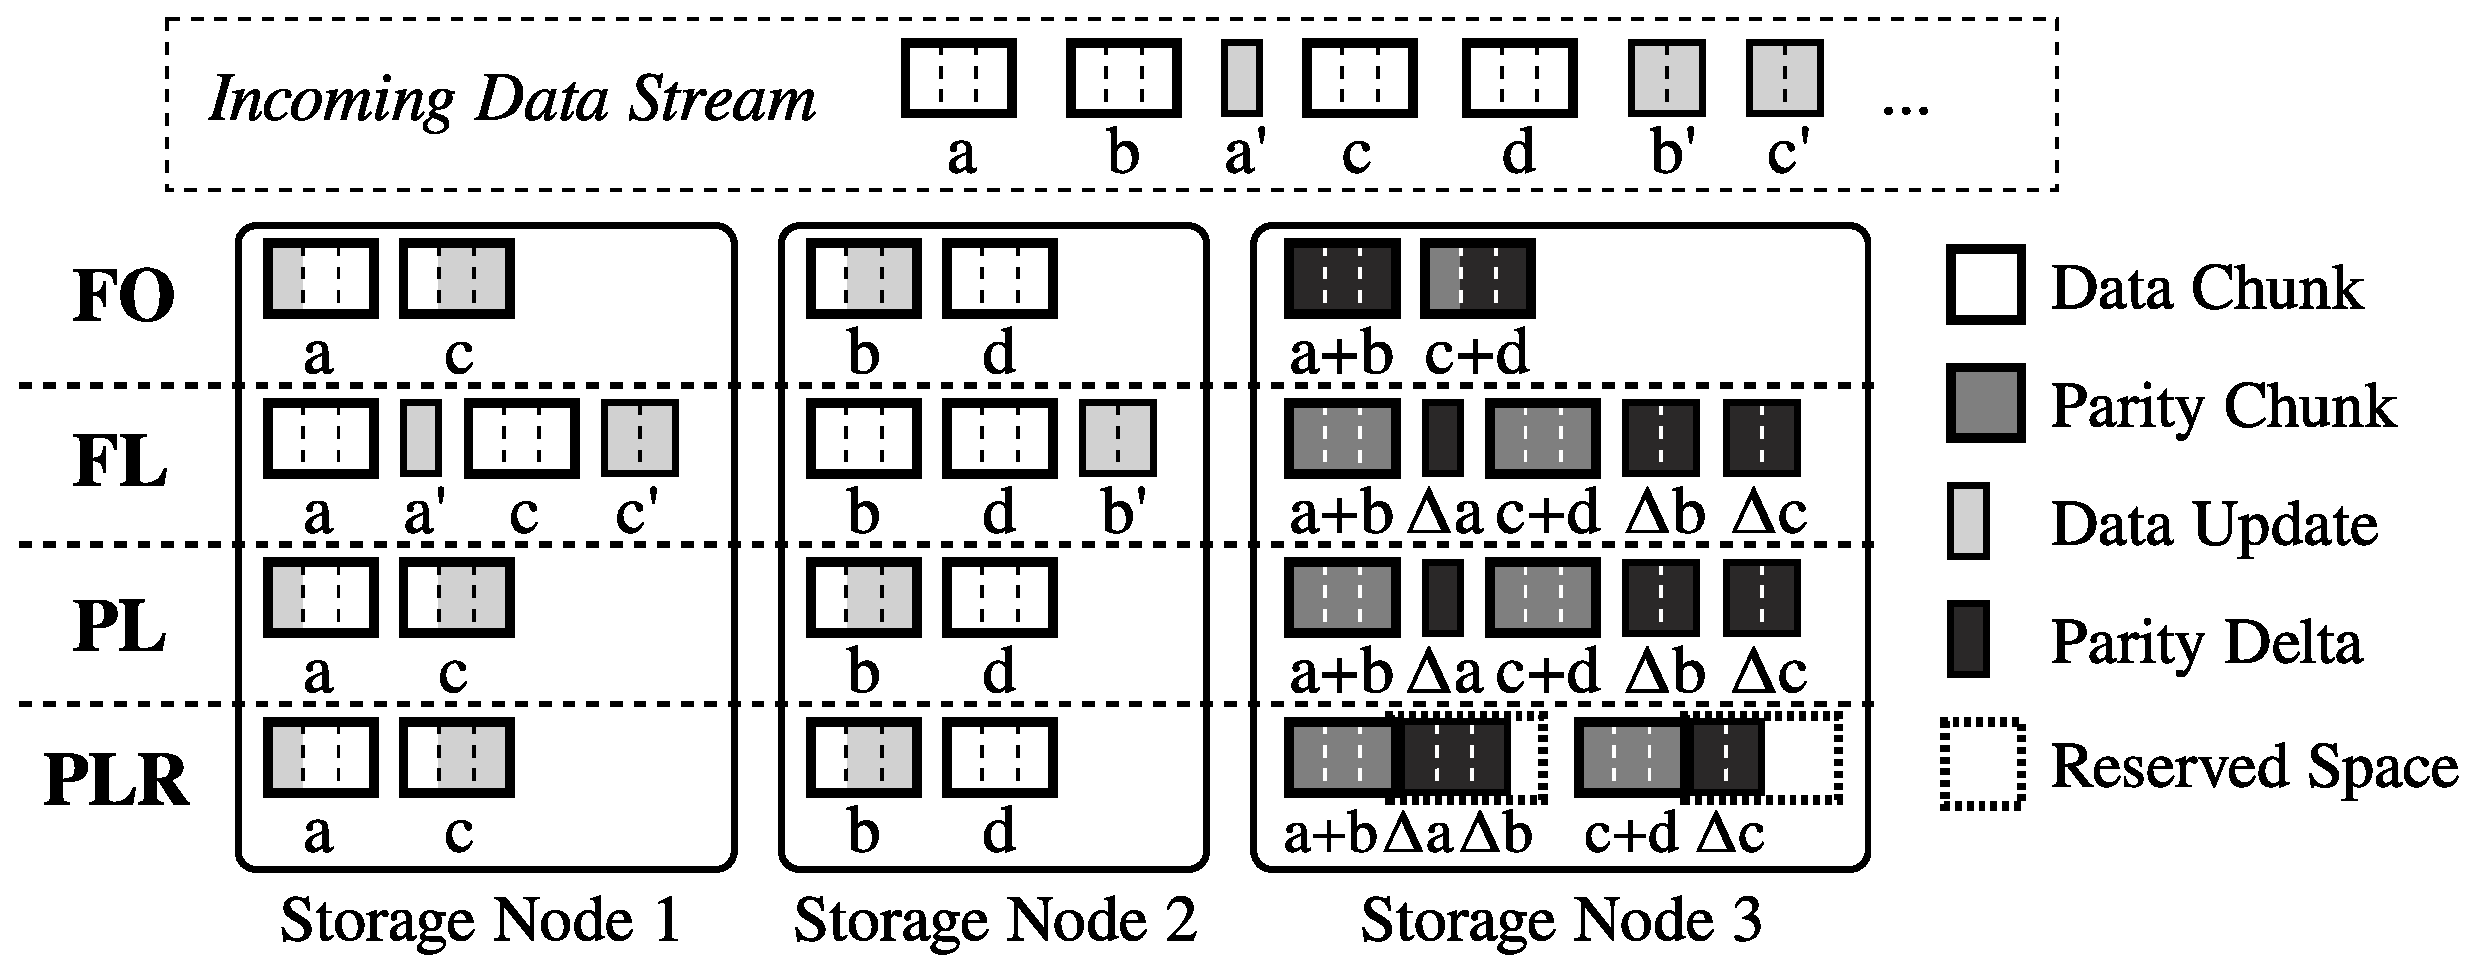
\includegraphics[width=4.8in]{figs/schemes_chunkflow}
%    \hspace{-3pt}
    \caption{Illustration on different parity update schemes.}
    \label{fig:schemes_chunkflow}
\end{figure*}


Figure~\ref{fig:schemes_chunkflow} illustrates the differences of the
delta-based approaches in \S\ref{sec:delta_based} and \PLR, using a
(3,2)-code as an example.  The incoming data stream describes the sequence of
operations: (1) write the first segment with data chunks \texttt{a} and
\texttt{b}, (2) update part of \texttt{a} with \texttt{a'}, (3) write a new
segment with data chunks \texttt{c} and \texttt{d}, and finally (4) update parts
of \texttt{b} and \texttt{c} with \texttt{b'} and \texttt{c'}, respectively.  We
see that \FO performs overwrites for both data updates and parity deltas; \FL
appends both data updates and parity deltas according to the incoming order; \PL
performs overwrites for data updates and appends parity deltas; and \PLR appends
parity deltas in reserved space. 

Consider now that we read the up-to-date chunk \texttt{b}.  \FL incurs a disk
seek to the update \texttt{b'} when rebuilding chunk \texttt{b}, as 
\texttt{b} and \texttt{b'} are in discontinuous physical locations on
disk.  Similarly, \PL also incurs a disk seek to the parity delta
\texttt{$\Delta$b} when reconstructing the parity chunk \texttt{a+b}. On the
other hand,  $\PLR$ incurs no disk seek when reading the parity chunk 
\texttt{a+b} since its parity deltas \texttt{$\Delta$a} and \texttt{$\Delta$b} are all placed
in the contiguous reserved space following the parity chunk \texttt{a+b}. 

\subsection{Determination of Reserved Space Size}
\label{sec:reserve_strategies}

Finding the appropriate reserved space size is challenging.  If the space is
too large, then it wastes storage space.   On the other hand, if the space is
too small, then it cannot keep all parity deltas.  

%Thus, before storing the
%coming delta, when the reserved space is full, a \textit{merge} operation is 
%first performed to apply the deltas in the reserved space to the parity
%chunk. In the worst case, the update performance can downgrade to the \FO
%approach if the parity chunk needs to be merged every time.

%The \PLR approach avoid the parity fragmentation by preallocating a reserved
%space. However, it also introduces merging overhead once the reserved space
%is full. Hence, we intend to minimize the number of merge operations since
%latency increases when updates are stalled during a merge.  Although using a
%larger reserved space can effectively prevents merging, it introduces
%unnecessary storage space overhead. 

%\red{the alternatives' name may be discussed}

A baseline approach is to use a fixed reserved space size for each parity
chunk, where the size is assumed to be large enough to fit all parity deltas.  
Note that this baseline approach can introduce
significant storage overhead, since different segments may have different
update patterns.  For example, from the Harvard NFS traces shown in
Table~\ref{table:harvard}, although $91.56\%$ of write requests are updates,
only around $12\%$ of files are actually involved.  This uneven distribution
implies that fixing a large, constant size of reserved space can imply
unnecessary space wastage. 

For some workloads, the baseline approach may reserve insufficient space to
hold all deltas for a parity chunk. There are two alternatives to handle extra
deltas, either logging them elsewhere like \PL, or \textit{merging} existing
deltas with the parity chunk to reclaim the reserved space.  We adopt the
merge alternative since it preserves the property of no fragmentation in
\PLR.

To this end, we propose a workload-aware reserved space management scheme that
dynamically adjusts and predicts the reserved space size. The scheme has
three main parts: 
(1) predicting the reserved space size of each parity chunk 
using the measured workload pattern for the next time interval, 
(2) shrinking the reserved space and releasing unused reserved space back to 
the system, and
(3) merging parity deltas in the reserved space to each parity chunk.
To avoid introducing small unusable holes of reclaimed space after shrinking,
we require that both the reserved space size and the shrinking size be of
multiples of the chunk size.  This ensures that an entire data or parity chunk
can be stored in the reclaimed space. 

\begin{algorithm}[t]
\DontPrintSemicolon
$\emph{reserved} \gets $\verb|DEFAULT_SIZE|\;
\While{$\rm{true}$}{
  \KwSty{sleep}$(\emph{period})$\;
  \ForEach{chunk \textbf{\emph{in}} parityChunkSet}{
  $\emph{utility} \gets $ \FuncSty{getUtility}$(\emph{chunk})$ \;
  $\emph{size} \gets $ \FuncSty{computeShrinkSize}$(\emph{utility})$ \;
    %$size \gets $ \KwSty{roundToChunk}$(size)$ \;
    \FuncSty{doShrink}$(\emph{size}, \emph{chunk})$  \label{line:deallocate} \;
    \FuncSty{doMerge}$(\emph{chunk})$ \;
  }
%  \del{$\emph{reserved} \gets$ \FuncSty{predict}$(\emph{parityChunkSet})$}% \;}
}
\caption{Workload-aware Reserved Space Management}
\label{alg:deallocate}
\end{algorithm}

Algorithm~\ref{alg:deallocate} describes the basic framework of our
workload-aware reserved space management.  Initially, we set a default
reserved space size that
is sufficiently large to hold all parity deltas.  Shrinking and
prediction are then executed periodically on each storage node.  Let
$\mathcal{S}$ be the set of parity chunks in a node. For every time interval
$t$ and each parity chunk $p\in \mathcal{S}$, let $r_t(p)$ be the reserved
space size and $u_t(p)$ be the reserved space utility.   Intuitively, $u_t(p)$
represents the fraction of reserved space being used.  We measure $u_t(p)$ at
the end of each time interval $t$ using exponential weighted moving average
in \texttt{getUtility}:
%
\begin{equation*} \label{eq:utility_now}
    u_t(p)  = \alpha \frac{\emph{use}(p)}{r_{t}(p)} + (1-\alpha)u_{t-1}(p),
\end{equation*} 
%
where $\emph{use}(p)$ returns the reserved space size being used during the
time interval, $r_{t}(p)$ is the current reserved space size for chunk
$p$, and $\alpha$ is the smoothing factor.  
%We set $\alpha =0.05$ by default as the smoothing factor.  
According to the utility, we decide the unnecessary space size $c(p)$ that can
be reclaimed for the parity chunk $p$ in \texttt{computeShrinkSize}.  Here, we
aggressively shrink all unused space $c(p)$ and round it down to be a multiple
of the chunk size:
%
\begin{equation*} \label{eq:shrink_size}
%    c_p = c_p^{*} - (c_p^{*}\bmod ChunkSize)
	c(p) = \left\lfloor\frac{(1-u_{t}(p))r_{t}(p)}{ChunkSize}\right\rfloor
	\times ChunkSize.
\end{equation*} 

The \texttt{doShrink} function attempts to shrink the size $c(p)$ from the
current reserved space $r_{t}(p)$. Thus, the reserved space $r_{t+1}(p)$ 
for $p$ at time interval $t+1$ is: 
$$
r_{t+1}(p) = r_{t}(p) - c(p).
$$
%
If a chunk has no more reserved space after shrinking (i.e., $r_{t+1}(p)
= 0$), any subsequent update requests to this chunk are applied in-place as
in \FO.

Finally, the \texttt{doMerge} function merges the deltas in the reserved space
to
the parity chunk $p$ after shrinking and resets $\emph{use(p)}$ to zero. Hence
we free the parity chunk from carrying any deltas to the next time interval,
which could further reduce the reserved space size.  The merge operations
performed here are off the update path and have limited impact on the overall
system performance. 

%\del{Finally, we predict the reserved space size $R_{t+1}$ for the new parity
%chunks in the next time interval $t$ based on the average reserved space size
%of all existing parity chunks.  We also apply exponential weighted moving
%average on the prediction:}
%\begin{equation*} \label{eq:predict}
%    \del{
%R_{t+1} = \left\lfloor\frac{\beta \frac{\sum_{p\in \mathcal{S}}
%	r_{t+1}(p)}{|\mathcal{S}|} + (1-\beta) R_{t}}{ChunkSize}\right\rfloor
%	\times ChunkSize,
%%    P_{t+1} = P_{t+1}^{*} - (P_{t+1}^{*}\bmod ChunkSize)
%}
%\end{equation*} 
%\del{where $R_{t}$ is the predicted reserve space size for current time interval
%$t$ and we set $\beta = 0.05$ for the smoothing factor by default. We also
%adjust the prediction size to be a multiple of the chunk size.}

%heuristic we present for measurement and prediction in the framework is 
The above workload-aware design of reserved space management is simple and can
be replaced by a more advanced design.  Nevertheless, we find that this simple
heuristic works well enough under real-world workloads (see
\S\ref{eval:reserve_evaluation}). 

%\paragraph{Shrink with Merge.}
%We further propose the third strategy. 
%While the basic flow remains the same, 
%we perform a merge after shrinking the reserved space for each parity chunk, i.e. after
%line~\ref{line:deallocate} in Algorithm~\ref{alg:deallocate}. Hence we free the parity
%chunks from carrying any deltas to the next period, which 
%could further reduce the reserved space size.
%Also, performing merge operation off the update path have less impact on the
%entire system performance. Thus,
%we expected it to be more effective than the previous shrinking approach.

%Reserving space for parity chunk can be implemented by calling \texttt{fallocate}, which
%also supports shrinking the reserved space by specifying the
%\texttt{FALLOC\textunderscore FL\textunderscore PUNCH\textunderscore HOLE} flag.
%The overhead of calling \texttt{fallocate} for reserving or shrinking is
%negligible. Therefore, we expect the shrinking job does not hurt the system
%performance and we will evaluate the three strategies in
%\S\ref{sec:reserve_evaluation}. 

